% =============================================================
%  Faults on a symmetrical monopole — the two fault types, the
%  behaviour of the blocked half-bridge converter, and the transient
%  behaviour in the first milliseconds from the EMT benchmark of
%  CIGRE TB 832 [26]. Principles; the recorded values of one project
%  are in pugalur-thrissur.tex.
%  Figures: fig/tb832_fig6-11*.png (pole-to-ground fault at the DC
%  terminal), fig/tb832_fig6-13*.png (pole-to-pole fault) and
%  fig/tb832_fig6-16_cable_voltage_profile.png are the simulation
%  plots of [26], Section 6.4.2, extracted unchanged from the PDF
%  (pdfimages); the file names carry the figure number of the source.
% =============================================================
\subsection{Faults on a Symmetrical Monopole}
\label{sec:dcf-faults}

\subsubsection{The blocked half-bridge converter}
\label{sec:dcf-faults-converter}

A blocked half-bridge MMC is an uncontrolled diode rectifier between the AC
network and the DC circuit. Blocking the converter therefore neither
interrupts the fault current nor de-energises the DC circuit: the AC network
keeps feeding the fault through the diodes until the AC circuit breakers of
both stations open~[24]. Opening the AC circuit breakers is thus a mandatory
part of every DC fault clearing on this converter type, and the operating
times of mechanical switchgear, Section~\ref{sec:dcf-switchgear}, set the
pace of the recovery.

The fault detection and the blocking are independent of the fault location.
The IGBTs have to be switched off before the current exceeds their turn-off
capability, which rules out any selective decision at that stage~[24].
Selectivity --- in which zone the fault lies and whether a restart is
permitted --- is decided afterwards, while the fault is being cleared,
Section~\ref{sec:dcf-zones}. Once blocked, the sub-module capacitors are out
of the current path: the bus-to-pole voltage is lower than the sum of the
sub-module voltages of an arm, so the upper diodes of the sub-modules do not
conduct and the capacitor voltages stay at their values at the blocking
instant for the time frame of the breaker operation~[26].

\subsubsection{Pole-to-ground and pole-to-pole faults}
\label{sec:dcf-faults-types}

The symmetrical monopole is the DC equivalent of an ungrounded AC network.
Its ground reference is a high-impedance star-point unit, which grades the
two pole voltages against ground, so the two fault types behave
differently~[24]:

\begin{itemize}[itemsep=0.2em]
  \item \textbf{Pole-to-ground fault.} The high grounding impedance limits
        the fault current to the discharge of the faulted pole and the
        charging of the healthy one. The healthy pole, however, rises
        towards the full pole-to-pole voltage, limited by its arresters.
        The overvoltage persists after the AC circuit breakers open, because
        a cable section stores the charge, and has to be removed by a
        discharge unit before the restart.
  \item \textbf{Pole-to-pole fault.} There is no overvoltage, but a fault
        current fed by the diode rectifiers of both stations. After the AC
        circuit breakers open, this current freewheels through the converter
        diodes, driven by the energy in the converter reactors and the DC
        circuit, and decays with the $L/R$ time constant of the fault loop,
        which the fault impedance shortens. The deionisation time at the
        fault location starts only when the current has reached zero.
\end{itemize}

The two types therefore need different preparation before the restart: the
pole-to-ground fault needs the discharge of the healthy pole, the
pole-to-pole fault needs the decay of the freewheeling current. Both then
need the deionisation time of the arc before the DC circuit may be
re-energised. The specified recovery time of the pole-to-pole fault is
accordingly the longer of the two, Section~\ref{sec:dcf-sequence-attempts}.

\subsubsection{Transient behaviour in the first milliseconds}
\label{sec:dcf-faults-transient}

CIGRE TB~832 works both fault types through on an EMT benchmark~[26]: a
symmetrical monopole of half-bridge MMCs, two stations joined by a 200\,km
cable with DC arresters at both cable ends, the fault applied at the DC
terminal of one station (called here the near station) at $t = 1$\,s. The
quantities are in per unit of their rated values; the arrester energy in
per unit of the arrester rating. Table~\ref{tab:dcf-emt-events} gives the
order of events of the three cases.

\begin{table}[!ht]
  \centering
  \begin{tabular}{@{}l l l l@{}}
    \toprule
    \textbf{Case} & \textbf{Event}
      & \multicolumn{1}{c}{\textbf{Near station}} & \multicolumn{1}{c}{\textbf{Remote station}} \\
    \midrule
    Pole-to-ground, DC terminal
      & detection criterion     & DC voltage unbalance & DC overcurrent \\
      & detection               & 5.01\,ms  & 1.83\,ms \\
      & block                   & 5.11\,ms  & 1.93\,ms \\
      & AC circuit breaker open & 45.1\,ms  & 45.9\,ms \\
    \addlinespace
    Pole-to-pole, DC terminal
      & detection criterion     & DC overcurrent & DC overcurrent \\
      & detection               & 0.34\,ms  & 1.25\,ms \\
      & block                   & 0.44\,ms  & 1.35\,ms \\
      & AC circuit breaker open & 40.4\,ms  & 49.5\,ms \\
    \addlinespace
    Pole-to-ground, cable midpoint
      & detection criterion     & DC voltage unbalance & arm overcurrent \\
      & detection               & 4\,ms     & 0.84\,ms \\
      & block                   & 14\,ms    & 1.14\,ms \\
      & AC circuit breaker open & 44\,ms    & 31.1\,ms \\
    \bottomrule
  \end{tabular}
  \caption{Order of events after a DC fault on the EMT benchmark of
           TB~832, times after the fault instant~[26]}
  \label{tab:dcf-emt-events}
\end{table}

\paragraph{Pole-to-ground fault at the DC terminal.}
Figure~\ref{fig:dcf-emt-pg} shows the first 200\,ms. The voltage of the
faulted pole drops to zero. The healthy pole tends towards 2\,pu, because
the sum of the sub-module voltages in the ON state of each leg equals the
pole-to-pole voltage at the fault instant; the DC arresters at both cable
ends hold it below that value. The rate of rise depends on the cable: its
pole-to-ground capacitance, the mutual inductance of the screen and the
conductor resistance~[26]. The faulted pole discharges and the healthy pole
charges, which gives the current peaks of
Figure~\ref{fig:dcf-emt-pg}(b), about 2.3\,pu in the benchmark; their
magnitude depends on the cable and on the pre-fault current. The arm
currents, Figure~\ref{fig:dcf-emt-pg}(c), are shifted by the transient DC
current and reach slightly more than the nominal value; the peak stays
moderate because the switching impulse protective level of the arrester is
above the peak of the phase-to-phase internal bus voltage. The internal bus
voltages acquire a DC component, since the converter side is ungrounded and
the DC voltage is unbalanced. The sum of the sub-module voltages
decreases, because the number of sub-modules in the ON state does not
change while the arresters force the pole-to-pole voltage down. The energy
absorbed by the arresters, Figure~\ref{fig:dcf-emt-pg}(d), is higher on the
faulted side, about 0.5\,pu of the arrester rating against 0.2\,pu at the
remote station; its rate of rise falls once both converters are blocked, so
the later the converters block, the more energy the arresters absorb~[26].
Converter stations are often designed with a converter bus line-to-line
peak voltage above the knee point of the DC arresters, to reduce losses;
the AC network then feeds the pole-to-ground fault through the valve arms
until the AC circuit breakers of both stations are open~[26].

\begin{figure}[!ht]
  \centering
  \begin{minipage}[t]{0.49\linewidth}\centering
    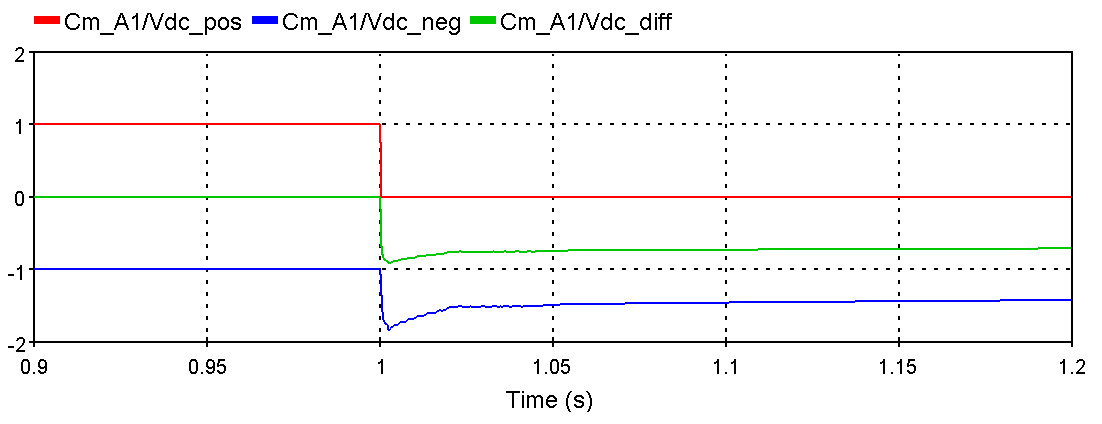
\includegraphics[width=\linewidth]{dc-fault-ride-through/fig/tb832_fig6-11a_pg_voltages.png}\\[-2pt]
    \footnotesize (a) pole-to-ground voltages, near station
  \end{minipage}\hfill
  \begin{minipage}[t]{0.49\linewidth}\centering
    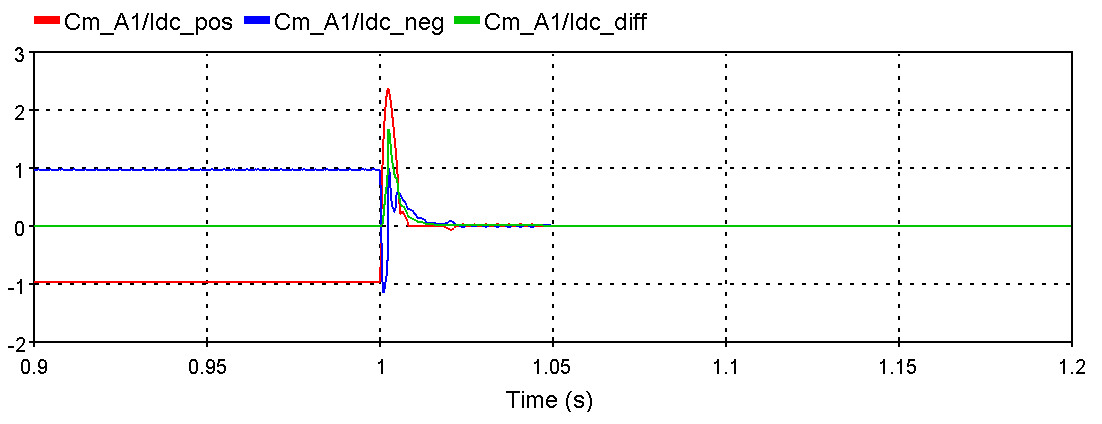
\includegraphics[width=\linewidth]{dc-fault-ride-through/fig/tb832_fig6-11b_pg_currents.png}\\[-2pt]
    \footnotesize (b) pole currents, near station
  \end{minipage}\\[6pt]
  \begin{minipage}[t]{0.49\linewidth}\centering
    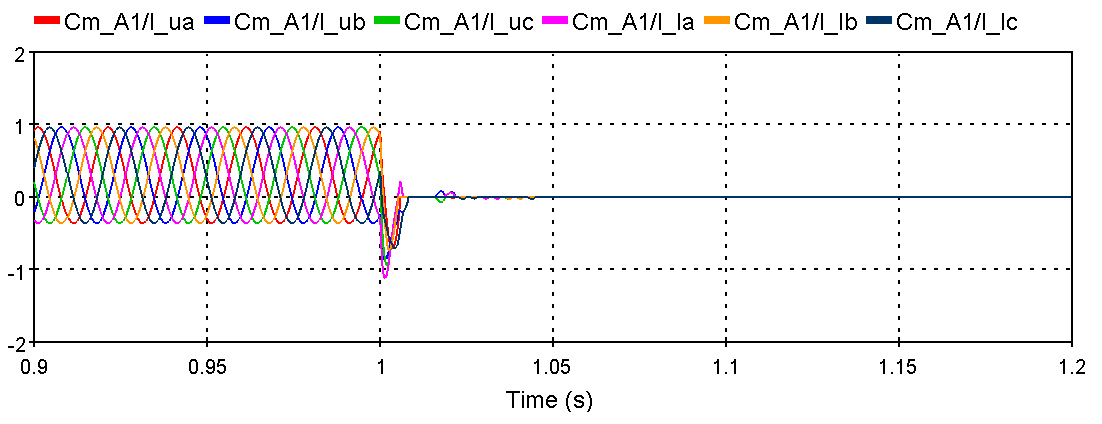
\includegraphics[width=\linewidth]{dc-fault-ride-through/fig/tb832_fig6-11c_pg_arm_currents.png}\\[-2pt]
    \footnotesize (c) arm currents, near station
  \end{minipage}\hfill
  \begin{minipage}[t]{0.49\linewidth}\centering
    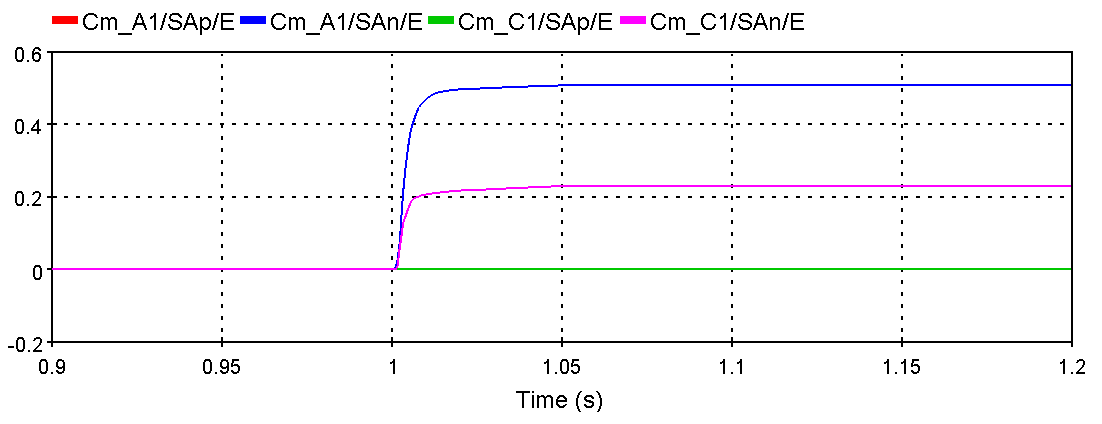
\includegraphics[width=\linewidth]{dc-fault-ride-through/fig/tb832_fig6-11h_pg_arrester_energy.png}\\[-2pt]
    \footnotesize (d) arrester energy, both stations
  \end{minipage}
  \caption{Positive pole-to-ground fault at the DC terminal of the near
           station on the EMT benchmark of TB~832, quantities in per unit,
           fault at $t = 1$\,s; the arrester energy in per unit of the
           arrester rating. Reproduced from~[26], Figure~6-11 (a), (b), (c)
           and (h)}
  \label{fig:dcf-emt-pg}
\end{figure}

\paragraph{Pole-to-pole fault at the DC terminal.}
Figure~\ref{fig:dcf-emt-pp} shows the same interval. At the fault location
the pole-to-pole voltage is zero at once; the remote station sees the
collapse about 1\,ms later, the propagation time over 200\,km of cable,
Figure~\ref{fig:dcf-emt-pp}(d). The DC current rises quickly, since the
sub-modules in the ON state are short-circuited by the fault, to about
8\,pu in the benchmark. Blocking does not reduce it: the inductances in the
DC current path hold the current, which then decays slowly through the
losses of the inductors and the diodes, and is still about 2\,pu 200\,ms
after the fault, Figure~\ref{fig:dcf-emt-pp}(b). With the converter blocked,
the bypass diodes of the upper and lower arms conduct until the arm current
crosses zero. Once the AC component of the fault current exceeds the DC
current established in an arm, that arm's current becomes positive only and
its diodes stop conducting; the sum of the upper or lower arm currents is
then no longer zero, an AC component appears in the DC fault current and the
DC fault current increases, Figure~\ref{fig:dcf-emt-pp}(c). When the AC
circuit breaker opens the AC contribution stops and the DC component decays
according to the impedance of the DC circuit~[26]. Seen from the AC side,
the blocked converter under a pole-to-pole fault is a reactor: the converter
bus voltages are those of the midpoint of a series reactor --- network
impedance plus transformer reactance on one side, arm reactor and smoothing
reactor on the other --- and the converter bus currents are those of a
three-phase shunt reactor with the transformer leakage reactance plus half
the arm reactance, about 4.5\,pu peak in the benchmark~[26].

\begin{figure}[!ht]
  \centering
  \begin{minipage}[t]{0.49\linewidth}\centering
    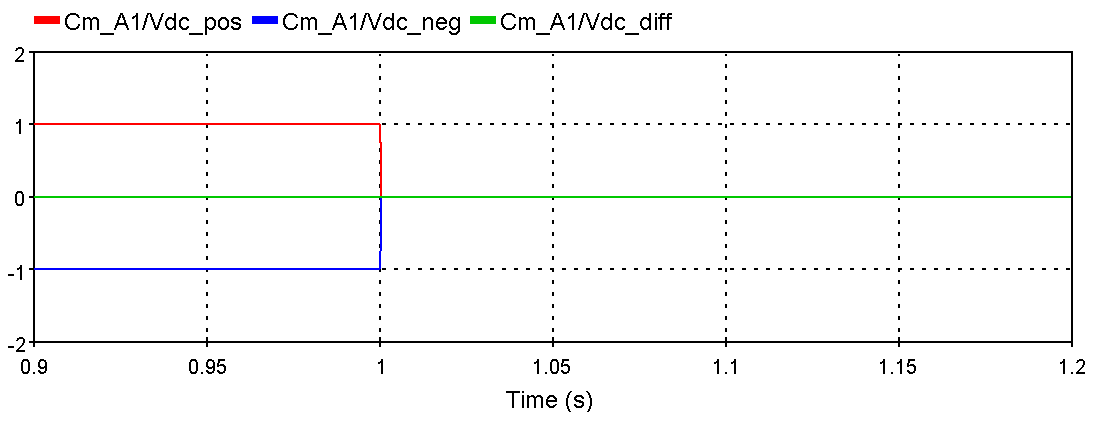
\includegraphics[width=\linewidth]{dc-fault-ride-through/fig/tb832_fig6-13a_pp_voltages.png}\\[-2pt]
    \footnotesize (a) pole-to-ground voltages, near station
  \end{minipage}\hfill
  \begin{minipage}[t]{0.49\linewidth}\centering
    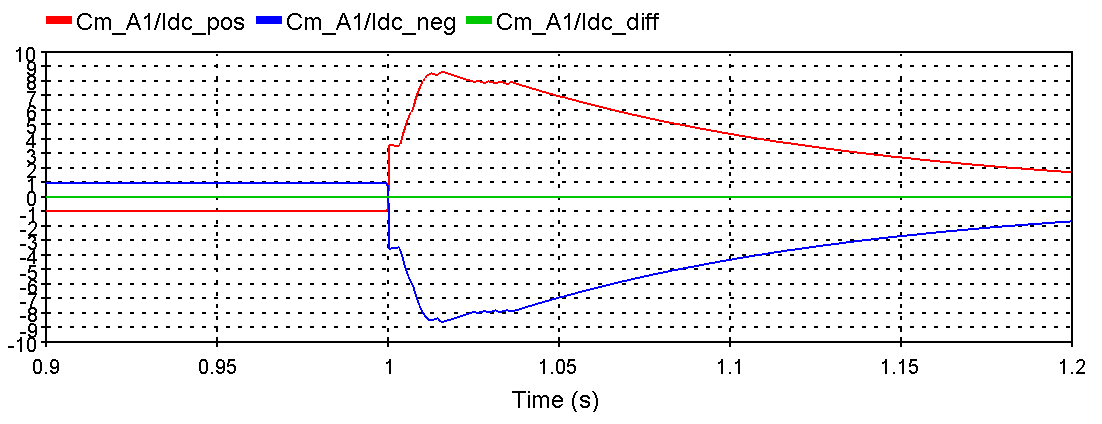
\includegraphics[width=\linewidth]{dc-fault-ride-through/fig/tb832_fig6-13b_pp_currents.png}\\[-2pt]
    \footnotesize (b) pole currents, near station
  \end{minipage}\\[6pt]
  \begin{minipage}[t]{0.49\linewidth}\centering
    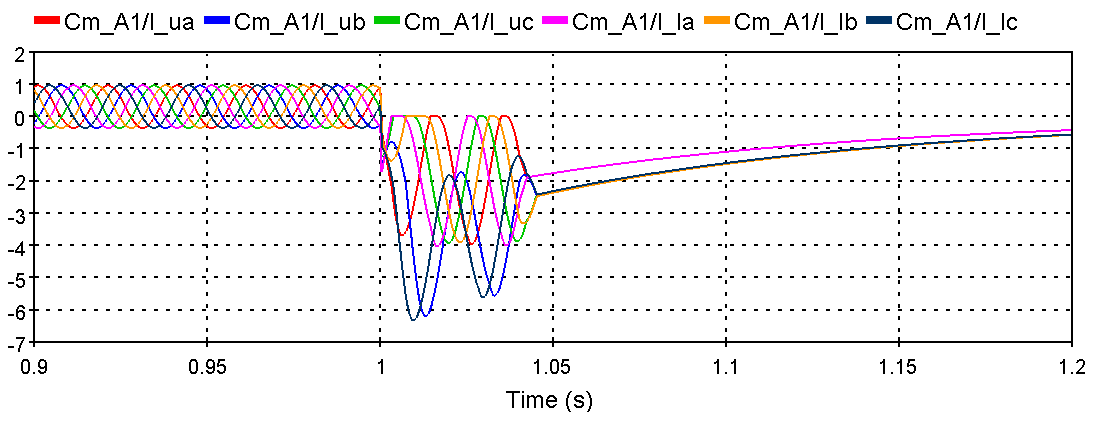
\includegraphics[width=\linewidth]{dc-fault-ride-through/fig/tb832_fig6-13c_pp_arm_currents.png}\\[-2pt]
    \footnotesize (c) arm currents, near station
  \end{minipage}\hfill
  \begin{minipage}[t]{0.49\linewidth}\centering
    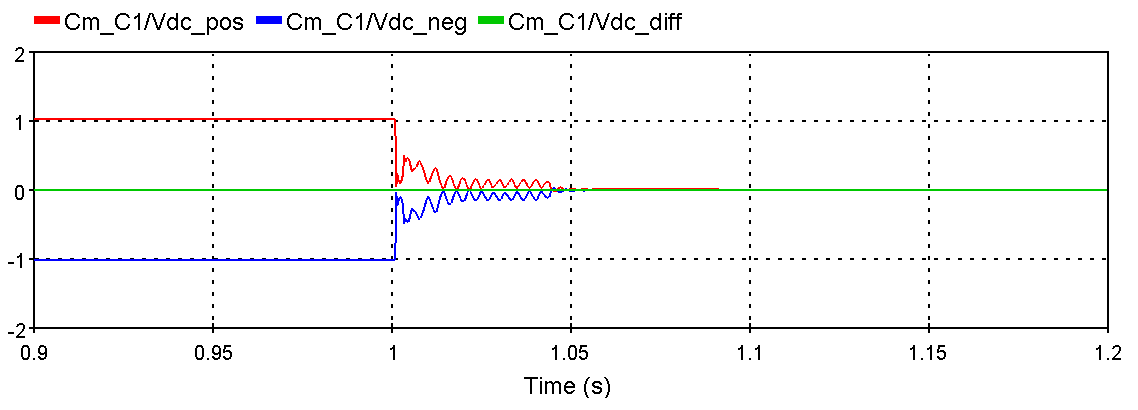
\includegraphics[width=\linewidth]{dc-fault-ride-through/fig/tb832_fig6-13g_pp_remote_voltages.png}\\[-2pt]
    \footnotesize (d) pole-to-ground voltages, remote station
  \end{minipage}
  \caption{Pole-to-pole fault at the DC terminal of the near station on the
           EMT benchmark of TB~832, quantities in per unit, fault at
           $t = 1$\,s. Reproduced from~[26], Figure~6-13 (a), (b), (c)
           and (g)}
  \label{fig:dcf-emt-pp}
\end{figure}

\paragraph{Pole-to-ground fault in the cable.}
For a fault at the midpoint of the 200\,km cable the voltage of the faulted
pole is forced close to zero at both terminals and the healthy pole is
limited to 1.8\,pu by the arresters; the rate of rise is lower than for the
terminal fault because of the added impedance in the fault path, and the
DC voltage starts to fall only when the AC circuit breakers are open on both
sides. The cable discharge current is superimposed on the pre-fault
current, so the peak is higher at the station that was feeding the cable:
in the benchmark that station exceeds its DC overcurrent threshold of
2.5\,pu and blocks after 1.14\,ms, while the other station blocks on DC
voltage unbalance after 14\,ms, Table~\ref{tab:dcf-emt-events}. The
sub-module voltages of the quickly blocked station are not affected, and
the arrester energy is lower than for a terminal fault because of the higher
impedance between fault and arresters~[26].

The peak voltage along a DC cable is not in general at its ends. It depends
on the cable parameters and on the fault location, through the travelling
waves and the arresters at the cable ends. In the benchmark of
Figure~\ref{fig:dcf-emt-cable}, for a fault at one terminal, the highest
pole-to-ground overvoltage of the healthy pole is reached close to the
middle of the cable, at 120\,km, and not at the terminals~[26]. The cable
insulation is therefore rated against the profile along the route, not
against the terminal voltages alone, Section~\ref{sec:dcf-ratings-cable}.

\begin{figure}[!ht]
  \centering
  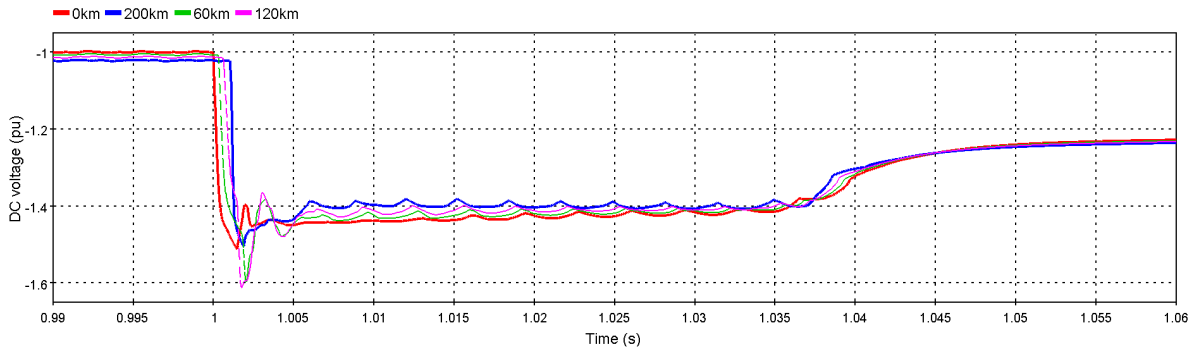
\includegraphics[width=0.7\linewidth]{dc-fault-ride-through/fig/tb832_fig6-16_cable_voltage_profile.png}
  \caption{Pole-to-ground voltage of the healthy pole at 0, 60, 120 and
           200\,km along the 200\,km cable of the TB~832 benchmark, fault at
           one terminal at $t = 1$\,s. Reproduced from~[26], Figure~6-16}
  \label{fig:dcf-emt-cable}
\end{figure}

\FloatBarrier
